% Tikz File 'mytikz.tex'
\documentclass{standalone}
%\input{../../Mod_base/grafica}
\input{../Mod_base/grafica}
\input{simboli_operatori}
\input{../Mod_base/unita_misura}
%\usetikzlibrary{...}
\begin{document}
\begin{tikzpicture}
\begin{axis}
[xmin=-6,xmax=6,ymin=-1,ymax=6, %grid,
axis x line=middle,xtick={-6,-5,...,6},ytick={-6,-5,...,6},
axis y line=middle,xlabel=$x$,ylabel=$y$]
%\addplot[samples=200] {(1^(x))};
\addplot [samples=200] {(1.2^(x))};
\addplot [samples=200] {(1.5^(x))};
\addplot [samples=200] {(2^(x))};
\end{axis}
%\node (a1) at (1,2) {$y=1^x$};
\node (a2) at (6,2.2) {$y=(\dfrac{6}{5})^x$};
\node (a3) at (6.2,4.2) {$y=(\dfrac{3}{2})^x$};
\node (a3) at (4.1,5) {$y=2^x$};
\end{tikzpicture}
\end{document}